\ffigbox[\FBwidth]{%
\caption{\centering Un graphe non orienté}\label{fig:td4_ex31_f1}
}{
    \fbox{
        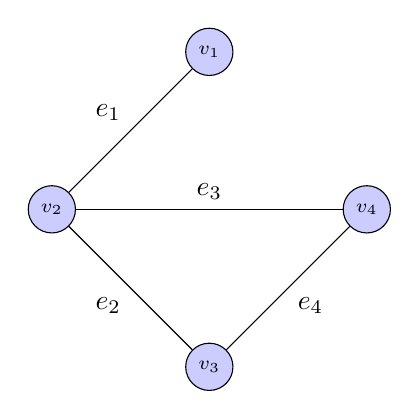
\begin{tikzpicture}[scale=1, main node/.style={circle, draw, fill=blue!20, inner sep=1pt, font=\scriptsize, minimum size=6mm, text=black}]
            % les sommets initiaux
            \node[main node] (v1) at (0,0) {\(v_1\)};
            \node[main node] (v2) at (-2,-2) {\(v_2\)};
            \node[main node] (v3) at (0,-4) {\(v_3\)};
            \node[main node] (v4) at (2,-2) {\(v_4\)};

            % les arcs avec capacités
            \draw (v1) to node[above left] {\(e_1\)} (v2);
            \draw (v2) to node[below left] {\(e_2\)} (v3);
            \draw (v2) to node[above] {\(e_3\)} (v4);
            \draw (v3) to node[below right] {\(e_4\)} (v4);

        \end{tikzpicture}
    }
}